Throughout the thesis we will use the following formulations of the system models in state-space representation.
All the linearized models will be represented as linear time invariant (\acrshort{lti}) systems, while the original system will be represented using nonlinear state-space models.

\subsection{Continues Space-State Model}
The generalized continues-time \acrshort{ss} representation of an \acrshort{lti} system can be formulated as follows
\begin{align}
    \dot{\mathbf{x}}(t) &= A_c \mathbf{x}(t) + B_c \mathbf{u}(t) \label{eq:continues_state_transition} \\
    \mathbf{y}(t) &= C \mathbf{x}(t) + D \mathbf{u}(t)  \label{eq:continues_measurement}
\end{align}
where \( \mathbf{x}(t) \) is the state vector at time \( t \), \( \mathbf{u}(t) \) is the control input, \( \mathbf{y}(t) \) is the measured output, and \( A_c \), \( B_c \), \( \transpose{C} \), and \( D \) are the system matrices derived from the linearized model.
For consistency we will use \( C \) defined as a row matrix.
\subsubsection{Continues Space-State Stochastic Model}
The generalized continues-time \acrshort{ss} stochastic model of a \acrshort{lti} system can be represented in the following form
\begin{align}
    \dot{\mathbf{x}}(t) &= A_c \mathbf{x}(t) + B_c \mathbf{u}(t) + \mathbf{w}(t) \label{eq:continues_state_transition_stochastic} \\
    \mathbf{y}(t) &= C \mathbf{x}(t) + D \mathbf{u}(t) + \mathbf{v}(t)  \label{eq:continues_measurement_stochastic}
\end{align}
where \( \mathbf{w}(t) \) is the process noise and \( \mathbf{v}(t) \) is the measurement noise, both assumed to be zero-mean Gaussian noise with known covariance matrices.
The stochastic model accounts for uncertainties in the system dynamics and measurements, making the model more realistic when simulating real-world scenarios. The implementation process is straight forward, as it only requires adding noise terms to the state transition and measurement equations.
Respectively, the process noise \( \mathbf{w}(t) \) and measurement noise \( \mathbf{v}(t) \) definition used within the thesis can be formulated using the Gaussian distribution as follows:
\begin{align}
    \mathbf{w}(t) &\sim \mathcal{N}(0, Q) \label{eq:process_noise} \\
    \mathbf{v}(t) &\sim \mathcal{N}(0, R)  \label{eq:measurement_noise}
\end{align}
where \( Q \in \mathbb{R}^{n \times n}\) is the process noise covariance matrix, \( R \in \mathbb{R}^{m \times m} \) is the measurement noise covariance matrix, \( n \) is the number of states of the system and \( m \) is the number of measurements. These matrices define the statistical properties of the noise affecting the system and measurements, respectively, and are crucial for the design and performance of state estimators such as the \acrshort{kf} and \acrshort{ekf}.
We can easily model Normal (Gaussian) noise using the following function:
\begin{equation}
    f(x) = \frac{1}{\sqrt{2 \pi \sigma^2}} e^{-\frac{(x - \mu)^2}{2 \sigma^2}}
\end{equation}
where \( \mu \) is the mean (expected value) and \( \sigma^2 \) is the variance of the distribution. In our case, both \( \mu \) values are set to zero, representing zero-mean noise.
\begin{equation}
    \mu = E[X] = \frac{1}{N} \sum_{i=1}^{N} X_i
    \label{eq:mean}
\end{equation}
where \( E[X] \) is the expected value of the random variable \( X \sim \mathcal{N}(\mu, \sigma^2) \), \( N \in \mathbb{N} \) is the total number of samples, and \( \mu \in \mathbb{R} \) is the mean. The variance \( \sigma^2 \) is calculated as:
\begin{equation}
    \sigma^2 = E[(X - \mu)^2] = \frac{1}{N} \sum_{i=1}^{N} (X_i - \mu)^2
    \label{eq:variance}
\end{equation}
\begin{equation}
    \sigma = \sqrt{\sigma^2}
    \label{eq:std_deviation}
\end{equation}
where \( \sigma \in \mathbb{R}^+ \) is the standard deviation, which quantifies the amount of variation or dispersion of a set of values around the mean.
As an example, if we want to simulate process noise with a standard deviation of \( 0.3 \) the variance \( \sigma^2 \) would be \( 0.09 \) based on \eqref{eq:variance}. The graphed representation of such noise is shown in Figure \figref{fig:gaussian_noise_example}.
\begin{center}
    \vbox{%
        \makebox[\textwidth][c]{%
            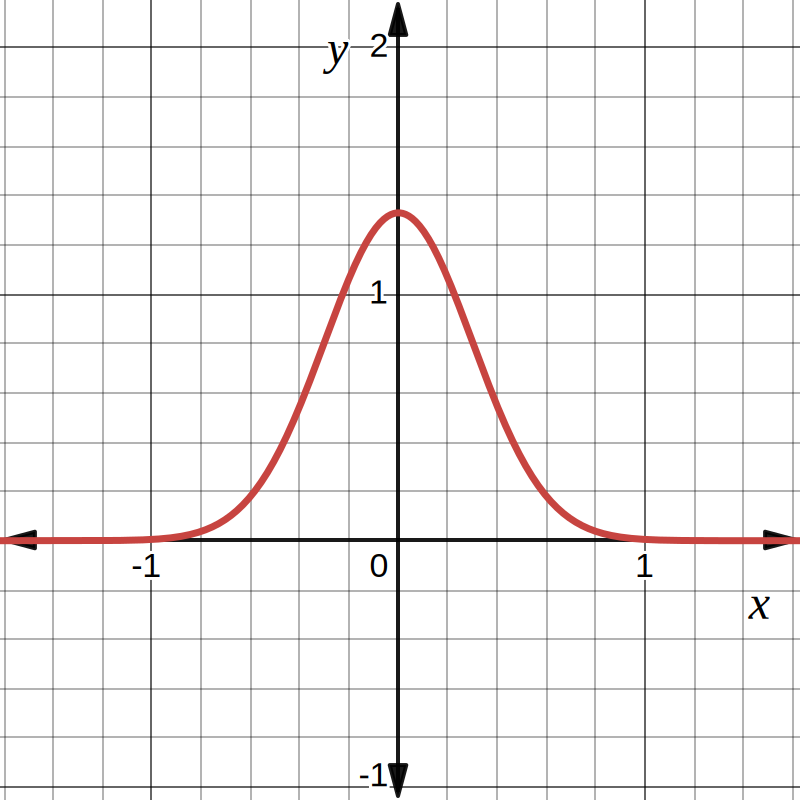
\includegraphics[width=0.7\textwidth]{norm_dist.pdf}
        }

        \figcaption{
            Graphical representation of Gaussian distribution with \( \mu = 0 \) and \( \sigma = 0.3 \).
        }
        \label{fig:gaussian_noise_example}
    }%vbox
\end{center}

The process of integrating these noise components into the following state-space models is essentially the same, as shown in equations \eqref{eq:continues_state_transition_stochastic} and \eqref{eq:continues_measurement_stochastic}.
Except when dealing with discrete-time models, where the noise terms need to be appropriately scaled based on the sampling period to ensure accurate representation of the noise characteristics in the discrete domain.
A change of notation is in order when tranforming continuous time to discrete time is required, thus instead of adding \( \mathbf{w}(t) \) and \( \mathbf{v}(t) \), we add \( \mathbf{w}_k \) and \( \mathbf{v}_k \) to the respective equations.

\subsection{Discrete State-Space Model}
The discrete-time \acrshort{ss} representation of an \acrshort{lti} system can be formulated as follows
\begin{align}
    \mathbf{x}_{k+1} &= A \mathbf{x}_k + B \mathbf{u}_k \label{eq:discrete_state_transition} \\
    \mathbf{y}_k &= C \mathbf{x}_k + D \mathbf{u}_k  \label{eq:discrete_measurement}
\end{align}
where \( \mathbf{x}_k \) is the state vector at discrete time step \( k \), \( \mathbf{u}_k \) is the control input, \( \mathbf{y}_k \) is the measured output, and \( A \), \( B \), \( \transpose{C} \), and \( D \) are the system matrices derived from the linearized model.

\subsection{Nonlinear Continues State-Space Model}
The nonlinear continues-time \acrshort{ss} model of the system can be represented as:
\begin{align}
    \dot{\mathbf{x}}(t) &= f(t, \mathbf{x}(t), \mathbf{u}(t)) \label{eq:nonlinear_continues_state_transition} \\
    \mathbf{y}(t) &= h(t, \mathbf{x}(t), \mathbf{u}(t)) \label{eq:nonlinear_continues_measurement}
\end{align}
where \( f \) and \( h \) are nonlinear functions that describe the system dynamics and output, respectively.

\subsection{Nonlinear Discrete State-Space Model}
The nonlinear discrete-time \acrshort{ss} model of the system can be represented as:
\begin{align}
    \mathbf{x}_{k+1} &= f(k, \mathbf{x}_k, \mathbf{u}_k) \label{eq:nonlinear_state_transition} \\
    \mathbf{y}_k &= h(k, \mathbf{x}_k, \mathbf{u}_k) \label{eq:nonlinear_measurement}
\end{align}
where \( f \) and \( h \) are nonlinear functions that describe the system dynamics and output, respectively.
